\chapter{Fundamentals}\label{chap:fundamentals}

In this chapter, I go into the basics that are important for my work. First, I give an overview of differential privacy, describe the underlying idea, formalise it and outline the most important mechanisms for applying it. I then describe the basics of federated learning, mention problems that the method has with skewed data distributions and discuss possible privacy models in federated learning.

\section{Differential Privacy}

%\begin{itemize}
%%	\item Anwendung von DP in the wild (\cite{erlingsson:2014, tezapsidis:2017, apple:2017}) -> steht in introduction
%	\item Randomized Response als anschauliches Beispiel? (ähnlich wie bei \cite[p.1]{erlingsson:2014}) 
%\end{itemize}

Differential privacy is a method that protects the privacy of individuals in interactive queries to databases. The underlying database itself is not changed, which distinguishes it from non-interactive privacy measures such as \textit{k-anonymity}. Instead, the query to the database is modified in such a way that the privacy of individuals is protected. 

It was formalised by \textcite{dwork:2006} after it was shown that privacy requirements of \textcite{dalenius:1977} are not feasible in practice. In \citeauthor{dalenius:1977}, the philosophy was that an attacker should not learn anything that he could not have learnt without access to the database. \citeauthor{dwork:2006} shows that this definition is not feasible due to auxiliary information that the attacker may possess. 

In an example from \citeauthor{dwork:2006}, there is a database that shows the average height of Lithuanian women and the height of individuals is sensitive information. If the attacker now has the auxiliary information \glqq{}Person X is two centimetres shorter than the average Lithuanian woman\grqq{}, then he learns the exact height of person X, regardless of whether the person is in the database or not. 

Instead, \citeauthor{dwork:2006} uses differential privacy, an approach that does not directly take into account the knowledge of the attacker, but rather whether the attacker can learn more about an individual for a particular query if they are in the underlying database.

Formally, differential privacy compares the probability of obtaining a similar query result if an individual is in a database or not. The closer these probabilities are to each other, the less an attacker can learn from the presence of the individual in the database and the higher the privacy. The definition from \cite{dwork:2006} is as follows:

\begin{definition}\label{def:eps-differential-privacy}
	\emph{\textbf{$\epsilon$-Differential Privacy}} A \textit{randomized mechanism} $\mathcal{M}: \mathcal{D} \rightarrow \mathcal{R}$ with domain $\mathcal{D}$ and range $\mathcal{R}$ satisfies $\epsilon$-differential privacy if for any two adjacent inputs $d$, $d' \in \mathcal{D}$ and for any subset of outputs $S \subseteq \mathcal{R}$ it holds that $$\Pr[\mathcal{M}(d) \in S] \leq e^{\epsilon} \Pr[\mathcal{M}(d') \in S]$$
\end{definition}

It should also be emphasised here that the definition makes no requirements on the databases $d, d'$, except that they are neighbouring. Typically, the following definition applies:
% Quelle hinzufügen? Bzw. klar machen warum ich sie hier explizit aufschreibe, nämlich in abgrenzung zu den User-adjacent datasets\cite{mcmahan:2018}
\begin{definition}\label{def:example-adjacency}
	\emph{\textbf{Example-adjacent datasets}} Two datasets $d$ and $d'$ are defined to be example-adjacent if $d'$ can be formed by adding or removing a single example from $d$.
\end{definition}

When referring to neighbouring data sets in this paper, this definition generally applies unless explicitly described otherwise.

A slightly weakened version of the definition adds a parameter $\delta$ that represents the probability that the privacy guarantees are not met. It should therefore be chosen to be very small \cite{dwork:2014}. This definition is relevant because the frequently used Gaussian mechanism does not fulfil the stricter $\epsilon$ differential privacy definition, but one still wants to work with it. It is also necessary for the \textit{Advanced Composition Theorem}.

\begin{definition}\label{def:eps-delta-differential-privacy}
	\emph{\textbf{$(\epsilon, \delta)$-Differential Privacy}} A \textit{randomized mechanism} $\mathcal{M}: \mathcal{D} \rightarrow \mathcal{R}$ with domain $\mathcal{D}$ and range $\mathcal{R}$ satisfies $(\epsilon, \delta)$-differential privacy if for any two adjacent inputs $d$, $d' \in \mathcal{D}$ and for any subset of outputs $S \subseteq \mathcal{R}$ it holds that $$\Pr[\mathcal{M}(d) \in S] \leq e^{\epsilon} \Pr[\mathcal{M}(d') \in S] + \delta$$
\end{definition}

There is also the Rényi differential privacy, which has a parameter $\alpha$ in addition to the $\epsilon$. It is important for many theorems, but is less illustrative and can always be converted into $(\epsilon, \delta)$-differential privacy, which is why I will not go into this definition any further here. It is true that a mechanism that fulfils $(\alpha, \epsilon)$-DP also always fulfils $(\epsilon + \frac{\log 1 / \delta}{\alpha - 1}, \delta)$-DP for $0 < \delta < \epsilon$ \cite{mironov:2017}.

In order for a query to fulfil differential privacy, noise is added to a query result of $\mathcal{M}$. The noise can be drawn from the Laplace or normal distribution, for example. The variance of the distribution from which the noise is drawn depends on the sensitivity of a query. This describes the greatest possible change in the query result that can occur by adding or deleting an entry \cite{dwork:2006}.

\begin{definition}\label{def:l1-sensitivity}
	\emph{\textbf{L1-Sensitivity}} For $\mathcal{M}: \mathcal{D} \rightarrow \mathcal{R}^{d}$, the L1-Sensitivity of $\mathcal{M}$ is 
	$$
	\Delta \mathcal{M} = \max_{d_1, d_2}{||\mathcal{M}(d_1) - \mathcal{M}(d_2)||}_1
	$$
	for all adjacent datasets $d_1$, $d_2$
\end{definition}

The distributions are selected depending on the application. For example, there is the Laplace or Gaussian mechanism for making numerical queries, such as the average of a database, private. The exponential mechanism is used for queries that are to return a result from a defined set. This rates the potential results using an scoring function.\cite{mcsherry:2007}

The definition of sensitivity varies slightly in the mechanisms, for example the Gaussian mechanism uses the $\ell_2$ norm instead of the $\ell_1$ norm, but the intuition that it is about the maximum deviation in the query result by an individual is always retained. In addition, the Laplace mechanism fulfils $\epsilon$-differential privacy, while the Gaussian mechanism only fulfils $(\epsilon, \delta)$-differential privacy.\cite[p.261ff]{dwork:2014}

The methods mentioned so far can be used to guarantee the privacy of individual requests. However, if multiple requests are made, the level of privacy must also decrease, as the average of the individual requests converges towards the true value at some point \cite[p.42]{dwork:2014}. A major advantage of differential privacy is that this reduction in privacy can be estimated. There are some composition theorems for this:

The \textit{Basic Composition Theorem} states that the $k$-fold application of $\epsilon_i$-DP mechanisms requires a privacy budget of $\epsilon = \sum_{i=1}^{k}\epsilon_i$. For the strict $\epsilon$-DP definition, this is the optimal estimate \cite{steinke:2022}. Nevertheless, the privacy budget grows linearly with the number of requests. 

The theorem can also be applied to $(\epsilon, \delta)$-DP, but there is also an asymptotically better estimate with the \textcite{Advanced Composition Theorem}. Details in regard to that can be found in \textcite{dwork:2010, steinke:2022}.
Mechanisms in which subsampling is performed, i.e. in which only a random subset of the database is analysed, can bring further privacy advantages \cite{mironov:2019, steinke:2022}.

In addition, results obtained by a mechanism that fulfils differential privacy can be further processed without further compromising privacy (\textit{post-processing}) \cite{dwork:2014}.

\subsection{Differential Privacy in Machine Learning}\label{sec:fund-dp-in-ml}

The goal of differential privacy in machine learning is to protect the privacy of the individual data points in the training data.
In this case, this does not refer to the protection of the database itself, but to preventing sensitive information from the training data from being found by third parties when the trained model is used. 

Attacks on machine learning models include \textit{Reconstruction Attacks}, \textit{Model Inversion Attacks} or \textit{Membership Inference Attacks}. With \textit{Reconstruction Attacks}, an attempt is made to restore original data using features. 
Even though most machine learning algorithms do not save features from training data directly, there are individual algorithms such as support vector machines that do and can therefore be exposed to these attacks \cite[p.9ff]{chang:2023}.

In \textit{Model Inversion Attacks}, an attempt is made to predict the input to a model based on the output. \textcite{fredrikson:2015} analysed APIs from machine learning as a service providers and carried out such an attack based on the responses of their models. To do this, they trained AI models that were able to recover sensitive attributes from surveys as well as input images for facial recognition. 
This worked particularly well with the examples used to train the providers' models and therefore poses a major risk for people who contribute training data to such models' training data. To minimise the effectiveness of the attack, \citeauthor{fredrikson:2015} suggest reducing the level of detail in the output. They show that the reconstructed image for face recognition becomes significantly worse if the probabilities that the image represents a specific person are sufficiently rounded. Alternatively, the output of the probabilities can be omitted and only the most probable class can be returned.

In particular, differential privacy can significantly reduce the effectiveness of \textit{Membership Inference Attacks}\cite{shokri:2017} \cite[p.14f]{chang:2023}. The aim of this attack is not to reconstruct input data, but to find out whether a data point was part of the training data based on the output of a trained model.

In general, the application of differential privacy in machine learning creates a trade-off between the usefulness and the privacy of the model (\textit{Privacy-Utility Trade-off}). For this reason, attempts are made in various ways to maximise the usefulness of the model. On the one hand, research is being conducted into better estimates of privacy costs \cite{dwork:2010, abadi:2016, mironov:2019}.In addition, algorithms are being developed that can achieve better results than others \cite{papernot:2017}. There is also work that deals with the model architecture itself, e.g. \textcite{papernot:2021} have researched the effect of activation functions on privacy parameters and were able to achieve new \textit{state-of-the-art} accuracies on MNIST, FashionMNIST and CIFAR10 with restricted activation functions.

Another research direction is the application of individual privacy budgets for individual users or data points. It can be based on empirical studies that suggest that different people have different privacy requirements for their data \cite{jensen:2005, acquisti:2005}. In \autoref{fund-idp} and the following chapters, I will shed further light on this line of research.

During the training itself, there are various points at which differential privacy can be applied to ensure privacy. Each point has various advantages and disadvantages, which I will outline below. An overview can be found in \autoref{fig:design_principles_dpml}.

\begin{figure}[tb]
	\centering
	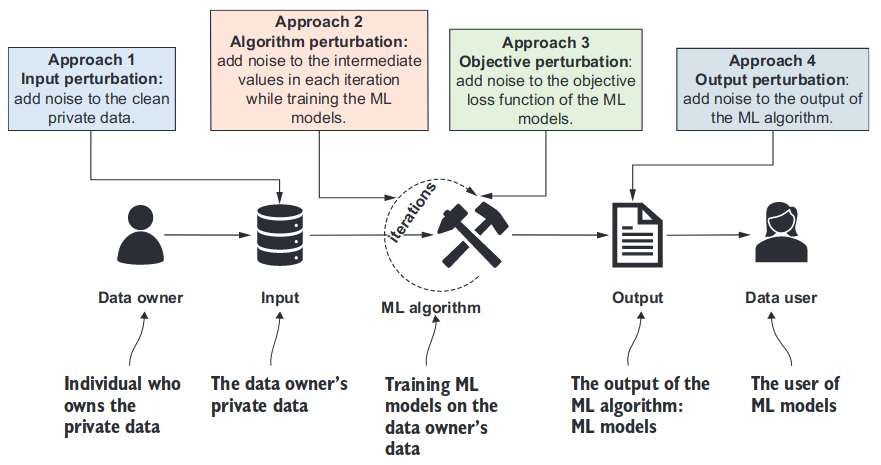
\includegraphics[width=0.9\textwidth]{Bilder/design_principles_dpml.png}
	\caption{Design principles of differentially private ML from \textcite{chang:2023}}
	\label{fig:design_principles_dpml}
\end{figure}

With \textit{input pertubation}, noise is added to the training data before the model is trained with it. This approach can be used without further changes to the training algorithm or the model, as the training algorithm then processes data that is already differential private, making it equivalent to \textit{post-processing}.The model can then be used again without any problems. However, a major disadvantage is that the queries on the training data generally have a high sensitivity and therefore a lot of noise has to be added.

The \textit{Algorithm Pertubation} is the most widely used method and is the basis for large libraries such as Opacus \cite{yousefpour:2021} and TensorFlow Privacy \cite{tfprivacy}. It can be used for iterative optimisation methods such as gradient descent or the power iteration method in principal component analysis (PCA).

When using this method in gradient descent (\texttt{DP-SGD}), differential privacy is applied to the gradients, i.e. these are usually truncated to a certain vector norm and then noise is added based on the now fixed sensitivity. Usually, significantly less noise needs to be added than with \textit{input pertubation} \cite{chang:2023}. The \textit{Privacy Loss} resulting from a training run can be determined using composition theorems.The \textit{Strong Composition Theorem}\cite{dwork:2010} was used for the estimation, but \textcite{abadi:2016} with the \textit{Moments Accountant} was able to provide a much more accurate estimate for the training of neural networks. 
The \textit{Strong Composition Theorem}\cite{dwork:2010} was initially used for the estimation, but \textcite{abadi:2016} were able to provide a much more accurate estimate for the training of neural networks with the \textit{Moments Accountant}. The trained model can also be published, as its weights fulfil the requirements of differential privacy. In particular, it not only protects against queries to the model providing information to an attacker, but also against the attacker downloading the model and analysing the model parameters, for example.

\textcite{shokri:2015} developed a decentralised training method for neural networks in compliance with differential privacy before \textcite{abadi:2016}. Similar to federated learning (see \autoref{fund-fl}), they propose distributed training. In their protocol, each participant shares only a subset of its parameters, which is why the privacy budgets are specified per model parameter. Parameters that have a larger gradient than a previously specified threshold are noised using the Laplace mechanism and then sent to the model server. 
However, the sum of the privacy budgets for an entire model can be very large\cite[p.10]{abadi:2016}.

\textit{Objective Pertubation} changes the objective function of the training.Instead of the data, noise is applied to this function during training.

With \textit{Output Pertubation}, a non-private model is trained and only the output of the model is noisy. This method has the major disadvantage that it cannot be used if the model is to be published.

One representative of this approach is \textit{PATE}\cite{papernot:2017}. Here, \textit{Teacher Models} are trained on disjoint subsets of the sensitive training data. The ensemble of these \textit{Teacher Models} then trains a \textit{Student Model} on a non-sensitive or public dataset. This data does not need to be labelled, as the trained \textit{Teacher Models} generate the labels. The advantage of this method is that it makes no demands on the models or the training process. The \textit{Teacher Models} also do not have to be trained privately, because the privacy is created by adding noise to the output of the ensemble with the \textit{Laplace mechanism}.

This corresponds to \textit{Output Pertubation}. As the repeated request of the \textit{Teacher Models} increases the loss of privacy, only a previously defined number of unlabelled data for the \textit{Student Model} is provided with labels. Only the label predicted with the highest confidence is used. This allows the \textit{Privacy Loss} to be estimated using composition theorems. The \textit{Student Model} trained in this way does not have this limitation and can be published.

Apart from the variance of the Laplace noise, the number of \textit{Teacher Models} is important for the trade-off between privacy and accuracy. A larger number of \textit{Teacher Models} reduces the loss of privacy, but also reduces their accuracy, as the amount of training data per \textit{Teacher Model} decreases.

\textcite{papernot:2017} evaluate \textit{PATE} on MNIST and SVHN. In the case of SVHN, they use the \textit{Extended Version} of the dataset and emphasise that the larger amount of training data available compensates for the additional complexity of the dataset. With 250 \textit{Teacher Models} they can achieve accuracies of $98\%$ (MNIST) and $90.66\%$ (SVHN). The result on MNIST can therefore beat \textcite{abadi:2016}.

The biggest disadvantage of PATE is that the algorithm requires non-private (potentially unlabelled) data, as the \textcite{Student Model} is trained non-privately. The algorithm of \textcite{abadi:2016} does not need this requirement.

\subsection{Individualized Differential Privacy}\label{fund-idp}

Motiviert von den verschiedenen Anforderungen und Präferenzen unterschiedlicher Personen an die Privatheit ihrer Daten haben \textcite{alaggan:2016} und wenig später unabhängig \textcite{jorgensen:2015} Arbeiten zu Differential Privacy mit individuellen Privacy Budgets veröffentlicht.

\textcite{alaggan:2016} definieren heterogene Differential Privacy im Kontext von Nutzerprofilen. In ihrer Arbeit individualisieren sie die Privacy durch das Anpassen der Sensitivität der Komponenten mit unterschiedlichen Budgets. Dazu erstellen sie eine \textit{Shrinkage Matrix}, mit der die Datenpunkte multipliziert werden. Die Matrix ist eine Diagonalmatrix, bei der die Diagonalelemente in $[0;1]$ liegen und abhängig von dem jeweiligen Privacy-Budget sind.

Ihr Ansatz ist jedoch für einige Funktionen nicht anwendbar, beispielsweise können das Minimum und die $\ell_0$-Norm nicht berechnet werden.

\textcite{jorgensen:2015} stellen einen Sampling Ansatz vor, mit dem beliebige DP-Algorithmen in einen Algorithmus mit individualisierter DP überführt werden können. Dabei wird der zugrundeliegende DP-Algorithmus als Black Box betrachtet und die Wahrscheinlichkeit, dass ein Tupel für den Algorithmus gezogen wird, davon abhängig gemacht, was der Nutzer als Privacy Budget gewählt hat.

In ihren Experimenten betrachten sie das gewählte Privacy Budget eines Nutzers als öffentliche Information. Dies kann als problematisch gewertet werden, da es theoretisch etwas über die Wichtigkeit einer Information aussagen kann. Sie rechtfertigen diesen Umstand damit, dass die Budgets nicht für ein Attribut gewählt werden sondern für ein Individuum mit potenziell vielen Attributen und diese Information daher nur etwas über die Person aussagt. Darüber hinaus plädieren sie dafür, einen Nutzer anstatt eines genauen Budgets eine bestimmte Privatheitsstufe mit angemessener Beschreibung (niedrig, mittel und hoch) zu spezifizieren, damit die Semantik der Budgets für Endnutzer verständlich bleibt.

Darüber hinaus zeigen sie ein weiteres Verfahren basierend auf dem \textit{Exponential Mechanism}. Diesen verändern sie dazu so, dass die Score-Funktion die individuellen Privacy Budgets mitbetrachtet. Sie wenden diesen Mechanismus auf \textit{Count}, \textit{Median} und \textit{Min} an, merken aber an, dass das Finden eines Algorithmus, der die angepasste Score-Funktion für beliebige Funktionen effizient berechnet, nicht trivial ist.

Sie weisen die Effektivität ihrer Verfahren in Experimenten nach, in denen sie beide Verfahren für \textit{Count} und \textit{Median} durchführen und eine \textit{Multiple Linear Regression} mit dem Sampling-Verfahren. Ihre Verfahren vergleichen sie mit Standard-DP Verfahren und bei \textit{Count} zusätzlich mit den Stretching-Verfahren aus \cite{alaggan:2016}. Die Privacy Budgets teilen sie in drei Gruppen mit aufsteigenden Privacy-Budgets auf (\textit{conservative}, \textit{moderate} und \textit{liberal}). Bei \textit{Count} leidet das Sampling-Verfahren dadurch, dass Elemente augeschlossen werden. Allerdings kann der angepasste \textit{Exponential Mechanism} gute Ergebnisse liefern und das Stretching-Verfahren deutlich schlagen. \textit{Median} ist verhält sich gegenüber dem Sampling deutlich resistenter, weshalb der Ansatz hier auch gute Ergebnisse erzielen kann und auch besser abschneidet als der modifizierte \textit{Exponential Mechanism}. 

Auch bei der linearen Regression kann der Sampling Ansatz das Verfahren von \cite{alaggan:2016} schlagen. Der modifizierte \textit{Exponential Mechanism} ist hier nicht anwendbar.

\section{Federated Learning}\label{fund-fl}

Federated Learning (FL) ist ein Optimierungsverfahren, bei dem einzelne Clients gemeinsam über mehrere Runden ein Modell trainieren, ohne dabei ihre eigenen Trainingsdaten mit anderen zu teilen. Auch wenn noch viele Fragen im Federated Learning offen sind und erforscht werden, wird es erfolgreich in Produktivumgebungen eingesetzt und stellt im Training mit besonders sensiblen Daten eine gute Alternative gegenüber dem klassischen zentralisierten Training dar \cite{hard:2018, ramaswamy:2020}.

Im Federated Learning gibt es einen Server, der den Ablauf des Trainings steuert und eine beliebige Anzahl von Clients, die das lokale Training auf ihren eigenen Daten durchführen. Der generelle Ablauf einer Trainingsrunde sieht wie folgt aus: 

\begin{enumerate}
	\item der Server initialisiert ein Modell und dessen Parameter (nur erste Runde) 
	\item \label{round-start} er wählt eine Menge von Clients aus, mit denen in dieser Runde das Modell trainiert werden soll
	\item das Modell wird an die ausgewählten Clients geschickt
	\item die Clients optimieren das Modell auf ihren eigenen Daten und schicken die aktualisierten Parameter zurück an den Server
	\item der Server aggregiert die Parameter der Clients und konstruiert daraus neue Modellparameter
	\item danach geht es in der nächsten Runde mit \autoref{round-start} weiter bis das Modell konvergiert oder die festgelegte Rundenzahl erreicht ist
\end{enumerate}

Die lokale Optimierung und die Aggregation der Updates variiert je nach Algorithmus. Die beiden Standardalgorithmen sind \texttt{FedAvg} und \texttt{FedSGD}\cite{mcmahan:2016}. Der wichtigste Unterschied ist, dass \texttt{FedAVG} die Clients mehrere Epochen auf ihren eigenen Daten trainieren lässt, während die Clients im \texttt{FedSGD} nur einen Schritt machen, bevor sie die aktualisierten Parameter wieder an den Server schicken. In beiden Algorithmen werden die Updates bei der Aggregation nach der Menge an Datenpunkten beim jeweiligen Client gewichtet.

Das verteilte Training kann vor allem zwei Probleme mit sich bringen: Zunächst kann der Zusatzaufwand für die Kommunikation sehr groß werden, gerade wenn über viele Runden hinweg trainiert wird. Zum anderen kann nicht angenommen werden, dass die Daten über die Clients hinweg unabhängig und gleichverteilt (i.i.d.) sind, was die Konvergenz der Algorithmen beeinträchtigen kann. \textcite{karimireddy:2020} versuchen diesem Problem zu begegnen, indem sie in ihrem Algorithmus die generelle Richtung, in die die Clients optimieren, an die Clients schicken und diese sie in ihre Updates einfließen lassen.

Die Anwendungsfälle von Federated Learning können variieren: Zum einen gibt es das \textit{Cross-device Federated Learning} und zum anderen das \textit{Cross-silo Federated Learning}\cite{kairouz:2021}. 

Ersteres entspricht dem Fall, dass die Clients eine Vielzahl von mobilen oder IoT-Geräten sind. Hierbei sind die Clients sehr unzuverlässig, zum Beispiel kann der Empfang zu schlecht werden, ein Gerät ausgeschaltet werden oder wegen einem zu niedrigen Akkustand ungeeignet für die Teilnahme am Training sein. All dies kann von dem Server nicht beeinflusst werden, also muss das Trainingsverfahren mit solchen Ausfällen zurecht kommen. Darüber hinaus kann die Menge der Clients von dem Server nicht verlässlich indiziert werden, da Geräte auch dauerhaft ausfallen können, zum Beispiel wenn ein Mobiltelefon kaputt geht oder ein neues gekauft wird und deshalb laufend neue Geräte hinzukommen können.

Bei dem \textit{Cross-silo Federated Learning} geht es vor allem um das Trainieren von Modellen zwischen unterschiedlichen Datencentern oder Organisationen. Die Motivation hierbei ist vor allem, dass es ein gemeinsames Interesse mehrerer Parteien an aussagekräftigen Modellen gibt, die zugrundeliegenden Trainingsdaten aber nicht den anderen Organisationen bereitgestellt werden sollen. Hierbei ist die Ausfallsicherheit der Clients deutlich höher als beim \textit{Cross-device Federated Learning} und auch die Menge der Clients ist in der Regel bekannt.

Auch der Server selbst kann bei einer sehr großen Zahl an Clients zu einem Bottleneck werden.\cite[p.11]{kairouz:2021} Daher wird ebenfalls an vollständig verteilten Trainingsverfahren geforscht, bei denen kein zentraler Server nötig ist (\textit{Fully-decentralized learning}).

\subsection{Data heterogeneity}\label{fund-fl-data-heterogenity}

Ein häufig beschriebenes Problem des Federated Learnings ist die Heterogenität der Trainingsdaten. Da die Daten von unterschiedlichen Parteien generiert werden ist eine zufällige Verteilung der abhängigen und unabhängigen Variablen in der Regel nicht gegeben. Diese Heterogenität kann sich auf verschiedene Arten ausdrücken, wie im folgenden beschrieben.

Die Daten auf den einzelnen Clients können Abhängigkeiten aufweisen, beispielsweise wenn sie in einer zeitlichen Abfolge sortiert vorliegen. Derartige Abhängigkeiten können aber durch das Durchmischen der einzelnen Datenpunkte gelöst werden. Eine solche Verzerrung wird \textit{Intra-Client Distribution Skew} genannt.

Die Verteilung der Features kann sich zwischen den Clients unterscheiden, auch wenn die Wahrscheinlichkeit der Labels gegeben der Features, $P(y|x)$, die gleiche ist. Beispielsweise könnte es sein, dass eine Person sehr viele Hundebilder auf ihrem Handy hat, weil sie ein Hund als Haustier hat und eine andere Person sehr viele Katzenbilder, weil sie mit einer Katze wohnt. Diese Art von Verzerrung heißt \textit{Feature Distribution Skew}

Umgekehrt kann sich auch die Verteilung der Labels auf den Clients unterscheiden, zum Beispiel aufgrund von regionalen Unterschieden. Beispielsweise können Kängurus fast nur in Australien beobachtet werden. In diesem Fall wird es als \textit{Label Distribution Skew} bezeichnet.

Darüber hinaus werden von \textcite{kairouz:2021} weitere Verzerrungen erwähnt. So kann es sein, dass sich die bedingten Wahrscheinlichkeiten von Features und Labels unterscheiden, beispielsweise sieht ein Haus in den USA anders aus als in Europa, in beiden Fällen ist es aber ein Haus (\textit{concept drift}). Andersherum kann es auch sein, dass die gleichen Features anders gelabelt sind, beispielsweise weil manche Daten auch für Menschen ununterscheidbar sind. Außerdem kann die Anzahl der Trainingsbeispiele von Client zu Client sehr stark variieren. 

\subsection{Privacy model in Federated Learning}\label{sec:pm-in-fl}
Auch wenn das Training von Modellen im Federated Learning verhindert, dass Trainingsdaten das eigene Gerät verlassen, sind Angriffe auf die trainierten Modelle weiterhin möglich. Das schließt die in \autoref{sec:fund-dp-in-ml} Attacken ein, aber es gibt auch weitere Arbeiten, die sich speziell mit Federated Learning befassen \cite{geiping:2020, wang:2019}. Die Anwendung von Differential Privacy im Federated Learning hat das Potenzial die mit den Attacken verbundenen Risiken zu mindern. Es gibt unterschiedliche Herangehensweisen, um Differential Privacy im Federated Learning umzusetzen.

% local vs global (trusted server), record vs user level
Die bisherige Definition von Differential Privacy geht davon aus, dass die Privatheit einzelner Datenpunkte in einer Datenbank geschützt wird. Im Federated Learning ist die Struktur der Daten eine andere: Es gibt viele Clients und es ist wichtig die Privatheit des ganzen Datensatzes eines Clients zu schützen. Es reicht nicht aus einzelne Zeilen seiner Daten zu schützen. Wenn die Menge der Daten aller Clients als Datenbank angesehen wird, kann die Definition der benachbarten Datensätze aus  \autoref{def:example-adjacency} dementsprechend angepasst werden:

\begin{definition}\label{def:user-adjacency}
	\emph{\textbf{User-adjacent datasets} \cite{mcmahan:2018}} Let $d$ and $d'$ be two datasets of training examples, where each example is associated with a user. Then, $d$ and $d'$ are \textbf{adjacent} if $d'$ can be formed by adding or removing all of the examples associated with a single user from d.
\end{definition}

Mit dieser Definition kann gewährleistet werden, dass die Anwesenheit oder Abwesenheit der Trainingsdaten eines Nutzers nur einen unmerklichen Einfluss auf die Modellparameter des am Ende vom Lernprozess veröffentlichten Modells hat \cite{mcmahan:2018}.

Darüber hinaus kann Differential Privacy auf zwei Arten angewendet werden: lokal oder global. Bei der globalen Anwendung erfüllt wie oben beschrieben das Modell am Ende Differential Privacy. Allerdings sind die Gradienten, die an den Server geschickt werden nicht privat, denn das nötige Rauschen wird nur auf das Modellupdate angewendet, das aus den Updates aller Clients aggregiert wird. Es muss also dem Server vertraut werden \cite[p.44]{kairouz:2021}.

Alternativ dazu ist die lokale Anwendung von Differential Privacy. Dabei muss das Rauschen hinzugefügt werden, bevor der Client sein Update an den Server schickt. Dem Server wird nicht mehr per se vertraut, stattdessen wird in der Regel angenommen, dass der Server "honest-but-curious" ist. Das bedeutet, dass er zwar die Aufgaben, die er in dem Protokoll hat, richtig umsetzt, aber gleichzeitig versucht, aus den Zwischenergebnissen Informationen zu extrahieren. Auch wenn dieser Ansatz konsequenter ist, hat sich in der Praxis allerdings gezeigt, dass er schwieriger umzusetzen ist, unter anderem, da Zwischenergebnisse stärker verrauscht werden \cite[p.54]{kairouz:2021}.

In meiner Arbeit lege ich den Fokus auf die globale Anwendung von Differential Privacy. In \autoref{chap:related-work} beschreibe ich der Vollständigkeit halber aber auch noch andere Verfahren, die Differential Privacy lokal anwenden.